\chapter{Theoretical and technical background}

\section{Correlation Structure}
\label{ap:Correlation}
In the book Gaussian Markov Random Fields~\cite{rue2005gaussian}, Rue and Held demonstrate that a strong correlation between the hyper-parameter $\mu$ and the latent field $\bm{x}$ can significantly slow down convergence when using samplers, in particularly Gibbs samplers. 
They consider the hierarchical model

\begin{subequations}
	\begin{align}
		\mu &\sim \mathcal{N}(0, 1) \\
		\bm{x} | \mu &\sim \mathcal{N}(\mu \bm{1}, \bm{Q}^{-1}),
	\end{align}
	\label{eq:rueMod}
\end{subequations}

and apply a Gibbs sampler based on the full conditional distributions
\begin{align}
	\mu^{(k)} | \bm{x}^{(k)} &\sim \mathcal{N} \left( \frac{\bm{1}^T \bm{Q} \bm{x}^{(k-1)}}{1 + \bm{1}^T \bm{Q} \bm{1}}, \, \left(1 + \bm{1}^T \bm{Q} \bm{1} \right)^{-1} \right) \\
	\bm{x}^{(k)} | \mu^{(k)} &\sim \mathcal{N}(\mu^{(k)} \bm{1}, \bm{Q}^{-1}).
\end{align}
As illustrated in Figure~\ref{fig:RueHeld}, when the sampler is restricted to steps only in the $\mu$-direction (horizontal axis) or the $\bm{x}$-direction (vertical axis), it requires many iterations to adequately explore the parameter space. 
This inefficiency arises from the high correlation between $\mu$ and $\bm{x}$, visible in Figure~\ref{fig:RueHeld} as a 'squeeze' of the distribution.
\begin{figure}[ht!]
	\centering
	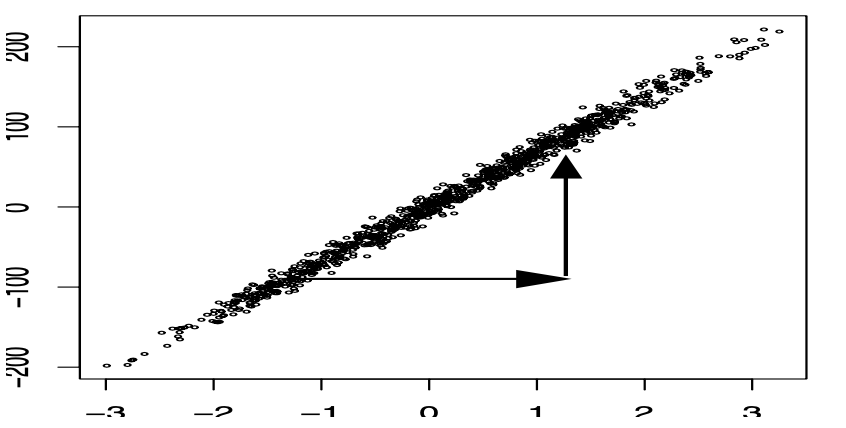
\includegraphics[width = \textwidth]{Figures/RueHeldBookFig.png}
	\caption[Correlation structure in between parameters and hyper-parameters]{The figure taken from~\cite[Figure 4.1 (b)]{rue2005gaussian}, shows samples from a marginal chain for $\mu$ and $\bm{1}^T \bm{Q} \bm{x}^{(k)}$ over 1000 iterations, based on the hierarchical model in Eq.~\ref{eq:rueMod}, with an autoregressive process encoded in $\bm{Q}$. The algorithm updates $\mu$ and $\bm{x}$ successively from their full conditional distributions. The plot displays $(\mu^{(k)}, \bm{1}^T \bm{Q} \bm{x}^{(k)})$, with $\mu^{(k)}$ on the horizontal axis and $\bm{1}^T \bm{Q} \bm{x}^{(k)}$ on the vertical axis. The slow mixing and convergence of $\mu$ result from its strong dependence on $\bm{1}^T \bm{Q} \bm{x}^{(k)}$, while the sampler permits only axis-aligned (horizontal and vertical) and does not allow diagonal moves, as illustrated by the arrows.}
	\label{fig:RueHeld}
\end{figure}

A solution to the slow mixing problem is to update $(\mu, \bm{x})$ jointly.
Since here $\mu$ is one dimensional, effectively only marginal density of $\mu$ is needed.
\begin{align}
	\mu^{\star}  &\sim q (\mu^{\star}|	\mu^{(k-1)} ) \\
	\bm{x}^{(k)} | \mu^{\star} &\sim \mathcal{N} (	\mu^{\star}\bm{1}, \bm{Q}^{-1}) 
\end{align}
With a simple MCMC algorithm targeting  $ \mu$ one can explore the sample space efficiently and only draw a corresponding sample for $\bm{x}$ from its full conditional once, for instance, the proposal $\mu^{\star}$ has been accepted.

\section{On the Monte-Carlo Error and Integrated Autocorrelation time}
\label{ap:IATC}
To assess the error $\sigma^2$ of chain $\mathcal{M}_i$, we ignore systematic error due to initialisation bias (burn-in period), but we have to take into account that samples produced by any system or algorithm are correlated.
To derive the integrated autocorrelation time (IATC), we follow the lecture notes \cite{wolff2002LecNot}.
In general, the error of a Monte-Carlo-based estimate from a sample set $\mathcal{M}_i = \{\bm{x}^{(1)}, \dots,\bm{x}^{(k)},\dots, \bm{x}^{(s)},\dots, \bm{x}^{(N)}\} \sim \pi(\bm{x}|\bm{y})$ is:
\begin{align}
	(\sigma^{(i)})^2 = \text{var}(\bm{\mu}^{(i)}_{\text{samp}} ) =  \text{var}(\text{E}_{\bm{x}|\bm{y}} [h(\bm{x})]) = \Bigg( \frac{1}{N} \sum_{k=1}^{N} h(\bm{x}^{(k)}) - \bm{\mu}^{(i)} \Bigg)^2 \, .
\end{align}
Expanding this summation, we see that
\begin{align}
	(\sigma^{(i)})^2 = \frac{1}{N^2} \sum_{k,s=1}^{N} \Gamma(k-s)
\end{align}
with the auto correlation coefficient $\Gamma(k-s) =  \big( h(\bm{x}^{(k)}) - \bm{\mu}^{(i)} \big) \big(h(\bm{x}^{(s)}) - \bm{\mu}^{(i)} \big)$.
Next we rewrite
\begin{align}
	\sum_{k,s=1}^{N} \Gamma(k-s) = \text{var}(\bm{\mu}^{(i)}_{\text{samp}})  \sum_{k,s=1}^{N} \frac{\Gamma(k-s)}{\Gamma(0)} =  \text{var}(\bm{\mu}^{(i)}_{\text{samp}}) \sum_{k,s=1}^{N}\rho(k-s)\, ,
\end{align}
with the normalised auto correlation coefficient $\rho(k-s) =  \Gamma(k-s)/ \Gamma(0)$ at lag $k-s$ and $\Gamma(0) = \text{var}(\bm{\mu}^{(i)}_{\text{samp}} )$ for $k=s$.
Typically $\Gamma(t)$ decays exponentially so that $\Gamma(t) \overset{t \rightarrow \infty }{ \propto} \exp\{ - t / \tau \}  $ and for positive $\tau$ and $N\gg \tau$ we can approximate
\begin{align}
	\sum_{k,s=1}^{N}\rho(k-s)  = N \sum_{t = -(N-1) }^{N-1} \Bigg(1- \frac{t}{N} \Bigg) \rho(t)  \approx N  \sum_{t = - \infty }^{\infty} \rho(t) \coloneqq 2 N \tau_{\text{int}}\, ,
\end{align}
see \cite{Sokal1997}, and define the IATC as in \cite[pp. 103-105]{wolff2002LecNot}.
If $\tau \gg 1$ one can show that $\tau_{\text{int}} \approx \tau$
\begin{align}
	\sum_{t = - \infty }^{\infty} \rho(t) =  1 + 2 \sum_{t = 1}^{\infty} \big(e^{-1/ \tau}\big)^t =  1 + 2 \frac{e^{-1/ \tau} }{1 - e^{-1/ \tau}} \approx  1 + 2 \frac{1 -1/ \tau }{1/ \tau} =  2 \tau -1 \approx 2 \tau_{int}
\end{align}
where we use the geometric power series $\sum^{\infty}_{n=0} x^n= 1/ (1+x)$ and the Taylor series $ e^x \approx 1+x$ for small $x$.
Consequently, the estimate for the Monte-Carlo error is:
\begin{align}
	(\sigma^{(i)})^2   \approx  \frac{\text{var}(h(\bm{x}) )}{N} \underbrace{\sum_{t = - \infty }^{\infty} \rho(t)}_{ \coloneqq 	2\tau_{\text{int}} } = \text{var}(h(\bm{x})) \frac{ 2 \tau_{\text{int}} }{N} \, , \label{eq:MCerr}
\end{align}
where we define the IACT provides a good estimate of how many steps the sampling algorithm needs to take to produce one independent sample.
More specifically, the effective sample size $\frac{ 2 \tau_{\text{int}} }{N}$ gives an estimate of how efficient a sampler is.

\section{Measure theory}
\label{ch:Mesure}
Recall the probability space $(\Omega, \mathcal{F}, \mathbb{P})$, where $\Omega$ denotes the sample space, and $\mathcal{F}$ is a collection of countable subsets $\{ A_n \}_{n \in \mathbb{N}}$ of $\Omega$. Each $A_n \subseteq \Omega$ is called an event, and a map $\mathbb{P} : \mathcal{F} \rightarrow \mathbb{R}$ is referred to as a measure.
In the following, we describe the conditions required for $\mathcal{F}$ to be a $\sigma$-algebra, and for $\mathbb{P}$ to qualify as a probability measure.
We refer to \cite{lawler2016notes} \cite{kopp2004measintprob} for further reading.

\subsection{Probability Measure}
For a probability measure, we require:
\begin{itemize}
	\item $\mathbb{P}(\Omega) = 1$ and $\mathbb{P}(\emptyset) = 0$
	\item $\mathbb{P}(A) \in [0,1]$
	\item $\mathbb{P}(\bigcup_{j \in \mathbb{N}} A_j )= \sum_{j \in \mathbb{N}}  \mathbb{P}(A_j)$ if we have pairwise disjoint sets or $A_i \cap A_j = \emptyset$ for $i \neq j $
\end{itemize}
In other words, the probability assigned to the entire sample space must be equal to one, $\mathbb{P}(\Omega) = 1$, and the probability of the empty set must be zero, $\mathbb{P}(\emptyset) = 0$. For any subset $A \subseteq \Omega$, the probability $\mathbb{P}(A)$ must lie between zero and one, i.e., $\mathbb{P}(A) \in [0,1]$.
If e.g. two subsets $A$ and $B$ are disjoint (i.e., $A \cap B = \emptyset$), then the probability of their union satisfies $\mathbb{P}(A \cup B) = \mathbb{P}(A) + \mathbb{P}(B)$.
This property must also hold for a countable sequence of disjoint sets $\{A_j\}_{j \in \mathbb{N}}$, such that $\mathbb{P}\left( \bigcup_{j \in \mathbb{N}} A_j \right) = \sum_{j \in \mathbb{N}} \mathbb{P}(A_j)$.

\subsection{$\sigma$-Algebra}
A collections of subsets $\mathcal{F}$ is called $\sigma$-algebra if:
\begin{itemize}
	\item $\emptyset, \Omega \in \mathcal{F} $,
	\item if $A \in \mathcal{F} $ then $A^C \coloneqq A / \Omega \in \mathcal{F}$
	\item if $A_1 , A_2, \dots  \in \mathcal{F} $ then $ \bigcup_{j \in \mathbb{N}}  A_j \in  \mathcal{F}$
\end{itemize}
In other words, the empty set $\emptyset$ and the entire sample space $\Omega$ must always be elements of $\mathcal{F}$. If a set $A \in \mathcal{F}$, then its complement $A^C = \Omega \setminus A$ must also be in $\mathcal{F}$. 
If, in terms of a probability measure, we are able to assign a probability $\mathbb{P}(A)$ to an event $A$, we must also be able to assign a probability to the event “not $A$”, i.e., $\mathbb{P}(A^C)$.
Finally, if a countable collection of sets $A_1, A_2, \dots \in \mathcal{F}$, then their union $\bigcup_{j \in \mathbb{N}} A_j$ must also be in $\mathcal{F}$. These three properties define the requirements for $\mathcal{F}$ to be a $\sigma$-algebra.

\clearpage
\section{Python Code}
\the\baselineskip

\begin{lstlisting}[language=Python, caption=Python example, escapeinside={"}{"}]
def MargBack(TTCore, univarGrid):
	''' Backward marginalisation, see Prop. "\ref{prob:BackMarg}" as in SIRT from Cui et al. "\cite{cui2022deep}" '''
	
	dim = len(univarGrid)
	B = dim * [None]  # coeffTensor
	B[-1] = TTCore[-1]
	R = [None] * dim
	C = [None] * dim
	
	for k in range(dim - 1, 0, -1):
		r_kmin1, n, r_k = np.shape(TTCore[k])
		# !! we set Lebesgue Measure to const = one
		M = np.identity(n) * (univarGrid[k][-1] - univarGrid[k][0])  # Mass matrix
		L = scy.linalg.cholesky(M)
		
		# construct Tensor C Eq. (27)
		C[k] = np.zeros((r_kmin1, n, r_k))
		for alpha in range(0, r_kmin1):
			for l in range(0, r_k):
				C[k][alpha, :, l] = B[k][alpha, :, l] @ L[:, :]
		
		# unfold along first coordinate and compute thin QR decomposition of C^T
		# Eq. (28)
		Q, R[k] = np.linalg.qr(C[k].reshape((r_kmin1, n * r_k), order='C').transpose(), mode='reduced')
		
		# compute next coefficient tensor
		# Eq. (29)
		r_kmin2, n, r_kmin1 = np.shape(TTCore[k - 1])
		B[k - 1] = np.zeros(np.shape(TTCore[k - 1]))
		for alpha_2 in range(0, r_kmin2):
		#for i in range(0, n):
			for l_1 in range(0, r_kmin1):
				B[k - 1][alpha_2, :, l_1] = TTCore[k - 1][alpha_2, :, :] @ R[k][l_1, :]

return B

\end{lstlisting}


\clearpage
\begin{lstlisting}[language=Python, caption=Python example, escapeinside={"}{"}]
def SIRT(seeds, SQTT, univarGrid, BackMarg, absError):
	''' do squared inverse rosenblatt transform SIRT as in Cui et al. "\cite{cui2022deep}" '''
	
	dim, numbSampl = seeds.shape
	sampls = np.zeros(seeds.shape)
	probVal = np.zeros(seeds.shape)
	Approx = np.zeros(seeds.shape[1])
	
	# lebesgue measure for qudrature "Eq. \ref{eq:lebesgueWeight}"
	WholeLebLam = np.zeros(dim)
	for k in range(0, dim):
		WholeLebLam[k] = (univarGrid[k][-1] - univarGrid[k][0])
	lamX = np.ones(dim)
	for k in range(1, dim):
		lamX[k - 1] = np.prod(WholeLebLam[k:])
	
	# error as in "Eq. \ref{eq:gamErr} \cite[Eq. (35)]{cui2022deep}"
	gamError = absError / np.prod(WholeLebLam)
	
	# sample from first dimension "\cite[Eq. (30)]{cui2022deep}"
	firstMarg = gamError * lamX[0] + np.sum(BackMarg[0][0, :, :] ** 2, 1)
	# cumulative distribution function, numerically normalised  
	# "Eq. \ref{eq:CurrCDF} \cite[Eq. (17)]{cui2022deep}"
	firstCDF = np.cumsum(firstMarg / np.sum(firstMarg))
	# draw samples as 'inverse transform'
	sampls[0] = np.interp(seeds[0], firstCDF, univarGrid[0])
	probVal[0] = np.interp(sampls[0], univarGrid[0], firstMarg / np.sum(firstMarg))
	
	# sample from other dimensions
	for n in range(0, numbSampl):
		# interpolate linear on grid in first dimension "Eq. \ref{eq:LinPol} \cite{dolgov2020approximation}"
		CurrApprCore = LinInterPolTT(SQTT[0], univarGrid[0], sampls[0][n])
		for d in range(1, dim):
			# marginal function condition on previous samples
			rank_min, gridSize, rank_pls = BackMarg[d].shape
			MargDep = np.zeros((BackMarg[d].shape))
			
			for r in range(0, rank_min):
				# condition on previous samples
				MargDep[r, :, :] = CurrApprCore[0, r] * BackMarg[d][r, :, :]
			
			# "Eq. \ref{eq:CurrMarg} \cite[Eq. (31)]{cui2022deep}"
			currMarg = gamError * lamX[d] + np.sum(np.sum(np.copy(MargDep), axis=0)** 2, axis=1)
			# "Eq. \ref{eq:CurrCDF} \cite[Eq. (17)]{cui2022deep}"
			currCDF = np.cumsum(currMarg / np.sum(currMarg)) 
			
			# draw sample as 'inverse transform'
			sampls[d][n] = np.interp(seeds[d][n], currCDF, univarGrid[d])
			probVal[d][n] = np.interp(sampls[d][n], univarGrid[d], currMarg / np.sum(currMarg))
			# piecewise polynomial interpolation, "Eq. \ref{eq:LinPol} \cite{dolgov2020approximation}"
			# multiply (condition) current dimension with previous samples
			CurrApprCore = np.copy(CurrApprCore) @ LinInterPolTT(SQTT[d], univarGrid[d], sampls[d][n])
	
	Approx[n] = gamError + CurrApprCore ** 2
	
	return sampls, probVal, Approx
\end{lstlisting}
\clearpage
\begin{lstlisting}[language=Python, caption=Python example, escapeinside={"}{"}]
def MargForw(TTCore, univarGrid):
''' Forward marginalisation, see Prop. "\ref{prob:ForMarg}", similar to backward marginalsiation as in  Cui et al. "\cite{cui2022deep}" '''
	# compute pre marginal coefficients sarting at dim = 1, k = 0
	BPre = dim * [None]  # coeffTensor
	LebLam = 1  # !! Lebesgue Measure
	BPre[0] = TTCore[0]
	RPre = [None] * dim
	CPre = [None] * dim
	
	for k in range(0, dim-1):
		r_kmin1, n, r_k = np.shape(TTCore[k])
		# !! we set Lebesgue Measure to const = one
		M = np.identity(n) * (univarGrid[k][-1] - univarGrid[k][0])  # Mass matrix
		L = scy.linalg.cholesky(M)
		
		# construct Tensor C "\cite[Eq. (27)]{cui2022deep}"
		CPre[k] = np.zeros((r_kmin1, n, r_k))
		for alpha in range(0, r_kmin1):
			for l in range(0, r_k):
				CPre[k][alpha, :, l] = BPre[k][alpha, :, l] @ L[:, :]
		
		# unfold along first coordinate and compute thin QR decomposition of C
		# "\ref{eq:RTE} \cite[Eq. (28)]{cui2022deep}"
		Q, RPre[k] = np.linalg.qr(CPre[k].reshape((r_kmin1 * n, r_k), order='C'), mode='reduced')
		
		# compute next coefficient tensor
		# "\cite[Eq. (29)]{cui2022deep}"
		r_k, n, r_kpls1 = np.shape(TTCore[k + 1])
		BPre[k + 1] = np.zeros(np.shape(TTCore[k + 1]))
		for alpha_1 in range(0, r_kpls1):
			for l_1 in range(0, r_k):
				BPre[k + 1][l_1, :, alpha_1] = RPre[k][l_1,:] @ TTCore[k + 1][:, :, alpha_1]
	
	return BPre
	
\end{lstlisting}


